\problemname{Wagon Sorting}

We have two sequences (or queues, to use a term familiar from computer science)
of railroad wagons, one starting at $Z_1$ and ending at $K_1$ and the other
starting at $Z_2$ and ending at $K_2$, as shown by the figure below. The arrows
indicate the direction into which the wagons can move.

\begin{figure}[h]
  \centering
  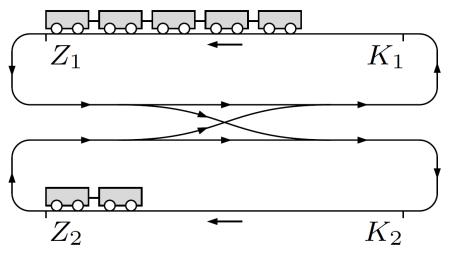
\includegraphics[width=0.6\textwidth]{wagons-queues}
\end{figure}

Each wagon has a unique numerical value, but we cannot access these values
directly. We can only deal with the wagons using a very limited set of
operations: we can check whether a queue is empty; we can move a wagon from the
start of one queue to the end of another queue, or even of the same queue; and
we can compare the values of the wagons at the start of both queues (and find
out which of them has the smaller value of the two).

Initially the first queue contains some unknown number ($n > 0$) of wagons in an
unknown order, while the second queue is empty. Our task is to use the
aforementioned operations so that at the end, all wagons will again be in the
first queue, but this time sorted in increasing order of their values.

\section*{Task}
This is an interactive task where your program will work with the wagons by
calling the following functions from a library provided by the organizers:
\begin{itemize}
  \item \texttt{void BeginSorting()} --- you must call this function at the
        beginning, before calling any other functions from the library.
  \item \texttt{bool IsEmpty(int q)} --- returns a logical value which indicates
        whether the queue $q$ is empty or not. The value $q$ must be either $1$
        or $2$.
  \item \texttt{void Move(int q, int r)} --- removes the first wagon from the
        start of the queue $q$ and transfers it to the end of the queue $r$. The
        values $q$ and $r$ must be from $\{1, 2\}$ and they are also allowed to
        be equal to each other. Both queues are large enough to accommodate all
        wagons, so there is never any question of the destination queue $r$
        being too full or anything of that sort.
  \item \texttt{int Compare()} --- compares the values of the wagons at the start
        of both queues, finds out which of them has the smaller value (note that
        no two wagons have the same value), and returns the number of the queue
        containing it. Hence this function always returns $1$ or $2$.
  \item \texttt{void DoneSorting()} --- you must call this function after you
        have finished sorting the wagons; after this you must not make any more
        calls to any functions from this library.
\end{itemize}

Your program must make exactly one call to \texttt{BeginSorting}, then $0$ or
more calls to \texttt{IsEmpty}, \texttt{Move}, and \texttt{Compare}, and finally
exactly one call to \texttt{DoneSorting}.

If your program doesn't call these functions in the correct order, or if it
passes values other than $1$ and $2$ as the arguments $q$ and $r$, or if it calls
\texttt{Move(q, r)} when the queue \texttt{q} is empty, or if it calls
\texttt{Compare} when at least one of the queues is empty, the run is rejected
and you score $0$ points for the current test case. The same happens if your
program uses the library correctly but the wagons are not sorted correctly at
the time of its call to \texttt{DoneSorting}.

To access the library, your program must include the header file
\texttt{wagonslib.h}. The header only declares the five library functions listed
above; your program provides its own \texttt{main}, which calls them.

The header file is provided as an attachment, together with
\texttt{wagonslib-public.cpp}, a simple implementation of the library that you
can use while developing your solution, and \texttt{wagons\_sample.cpp}, a small
example solution. To compile the library together with your program, simply add
its name as a parameter to the compiler, for example
\texttt{g++ foo.cpp wagonslib-public.cpp} if \texttt{foo.cpp} is the name of the
file containing your solution.

On the evaluation server, a different implementation of the library will be
used, so you should not make any assumptions about how exactly the
implementation works. You may, however, assume that it does not pollute the
global namespace with any declarations other than \texttt{BeginSorting},
\texttt{IsEmpty}, \texttt{Move}, \texttt{Compare}, and \texttt{DoneSorting}.

Your code must not read from the standard input or write to the standard output,
because those will be used by our implementation of the library on the
evaluation server to communicate with the rest of the evaluation environment.

\section*{Constraints}
\begin{itemize}
  \item The number of wagons $n$ is at least $1$ and at most $10\,000$.
\end{itemize}

\section*{Scoring}
On a particular run of your program, let $n$ be the number of wagons, and let $m$
be the total number of calls your program made to the functions
\texttt{IsEmpty}, \texttt{Move}, and \texttt{Compare}; then the performance of
your program on this run is evaluated by the value of $f_n(m)$, where $f_n$ is a
piecewise linear function defined as follows:

\noindent
\begin{tabular}{| l | l |}
  \hline
  $m$ & $f_n(m)$ \\ \hline
  $\leq 2n\lceil \log_2 n \rceil$ & $1$ \\ \hline
  $3n\lceil \log_2 n \rceil$ & $0.8$ \\ \hline
  $\geq n^2$ & $0.3$ \\ \hline
\end{tabular}

\noindent
In each of the ranges $[2n\lceil \log_2 n \rceil, 3n\lceil \log_2 n \rceil]$ and
$[3n\lceil \log_2 n \rceil, n^2]$, the function $f_n(m)$ is a linear function in
$m$.

In each subtask, your program will be run several times (on different initial
sequences of wagons); the number of points it will be awarded is defined as the
total number of points for that subtask multiplied by the smallest value of
$f_n(m)$ that your program will have achieved over all the runs in that subtask.

If your program doesn't sort the wagons correctly or doesn't adhere to the
aforementioned protocol in using the library, it will get $0$ points for the
whole subtask.

\noindent
\begin{tabular}{| l | l | p{12cm} |}
  \hline
  \textbf{Group} & \textbf{Points} & \textbf{Constraints} \\ \hline
  $1$ & $30$ & $30 \leq n \leq 100$ \\ \hline
  $2$ & $35$ & $800 \leq n \leq 1\,000$ \\ \hline
  $3$ & $35$ & $8\,000 \leq n \leq 10\,000$ \\ \hline
\end{tabular}

\section*{Example}
\noindent
\begin{tabular}{| l | l |}
  \hline
  \textbf{Call} & \textbf{Return value} \\ \hline
  \texttt{BeginSorting()} &            \\ \hline
  \texttt{Move(1, 2)}     &            \\ \hline
  \texttt{Compare()}      & $2$        \\ \hline
  \texttt{Move(1, 2)}     &            \\ \hline
  \texttt{IsEmpty(1)}     & \texttt{true} \\ \hline
  \texttt{Move(2, 1)}     &            \\ \hline
  \texttt{Move(2, 1)}     &            \\ \hline
  \texttt{DoneSorting()}  &            \\ \hline
\end{tabular}

\section*{Comment}
If the sequence of calls and return values took place as shown above, the
program will have sorted the two wagons correctly; but note that it has behaved
in a very risky fashion: if there had been just one wagon, the call to
\texttt{Compare} would have caused a runtime error!

The sample interaction shown below is the corresponding exchange between the
provided library and the judge. You never write it yourself --- the library does
--- but it may help you understand what the library is doing on your behalf.
